% \documentclass[letterpaper,12pt]{article}
\documentclass[11pt, a4paper]{article} 
% \documentclass[11pt,a4paper]{report}
\usepackage[margin=1in]{geometry}

\usepackage[utf8]{inputenc}
\usepackage{amsmath}
\usepackage{microtype}
\usepackage{graphicx}
% \usepackage{subcaption}
\usepackage{booktabs}

\usepackage{hyperref}
\hypersetup{
    colorlinks=true,
    citecolor=blue,
    linkcolor=red, % blue
    filecolor=magenta,      
    urlcolor=cyan,
}

% \usepackage{xcolor}
% \usepackage[dvipsnames]{xcolor}
% \usepackage{algorithm, algorithmic}
% \usepackage{algpseudocode}

% \usepackage{thm-restate}
% \declaretheorem[name=Theorem, sibling=theorem]{rThm}
% \declaretheorem[name=Lemma, sibling=theorem]{rLem}
% \declaretheorem[name=Corollary, sibling=theorem]{rCor}
% \declaretheorem[name=Proposition, sibling=theorem]{rPro}

\usepackage{graphicx} % more modern
\usepackage{subfigure}
\usepackage{multirow}
\usepackage{mathtools}
\usepackage{relsize}
\usepackage{url}
\usepackage{nicefrac}
\usepackage{xspace}
\usepackage{algorithm}
\usepackage{algorithmic}
\usepackage{multicol}
\usepackage{float}
\usepackage{bbm}


\usepackage[dvipsnames]{xcolor}
\usepackage{pifont}
\newcommand{\cmark}{{\color{PineGreen}\ding{51}}}%
\newcommand{\xmark}{{\color{BrickRed}\ding{55}}}%

\usepackage[utf8]{inputenc} % allow utf-8 input
\usepackage[T1]{fontenc}    % use 8-bit T1 fonts
\usepackage{hyperref}       % hyperlinks
\usepackage{url}            % simple URL typesetting

\usepackage{nicefrac}       % compact symbols for 1/2, etc.
\usepackage{microtype}      % microtypography

 % style
% \usepackage{fullpage}
\usepackage{layout}
\usepackage{multirow}
% \usepackage{cases}

% ams
\usepackage{amsfonts}
\usepackage{amsmath}
\usepackage{amsthm}
\usepackage{amssymb} % NOT COMATIBLE WITH svjour3

% shaded theorems
\usepackage{mdframed}
\usepackage{thmtools}

\usepackage[font=normalsize, labelfont=bf]{caption}


\newcommand{\OPT}{\texttt{OPT}}

\newcommand{\eps}{\varepsilon}
\newcommand{\reals}{\mathbb{R}}
\newcommand{\note}[1]{\textcolor{red}{#1}}
\newcommand{\ip}[2]{\left\langle #1, #2\right\rangle}
\newcommand{\nlsum}{\sum\nolimits}

\DeclareMathOperator{\Ocal}{\mathcal{O}}
\DeclareMathOperator{\sign}{sign}

%%% Basic sets
\newcommand{\R}{\mathbb{R}} % Reals
\newcommand{\N}{\mathbb{N}} % Naturals
\newcommand{\C}{\mathbb{C}} % Reals
\newcommand{\U}{\mathbb{U}} % Naturals

\newcommand{\Sam}{\mathbb{S}}


\newcommand{\fs}{f^\star} 
\newcommand{\xs}{x^\star} 

% caligraphic
\newcommand{\cA}{{\cal A}}
\newcommand{\cB}{{\cal B}}
\newcommand{\cC}{{\cal C}}
\newcommand{\cD}{{\cal D}}
\newcommand{\cE}{{\cal E}}
\newcommand{\cF}{{\cal F}}
\newcommand{\cG}{{\cal G}}
\newcommand{\cH}{{\cal H}}
\newcommand{\cJ}{{\cal J}}
\newcommand{\cK}{{\cal K}}
\newcommand{\cL}{{\cal L}}
\newcommand{\cM}{{\cal M}}
\newcommand{\cN}{{\cal N}}
\newcommand{\cO}{{\cal O}}
\newcommand{\cP}{{\cal P}}
\newcommand{\cQ}{{\cal Q}}
\newcommand{\cR}{{\cal R}}
\newcommand{\cS}{{\cal S}}
\newcommand{\cT}{{\cal T}}
\newcommand{\cU}{{\cal U}}
\newcommand{\cV}{{\cal V}}
\newcommand{\cX}{{\cal X}}
\newcommand{\cY}{{\cal Y}}
\newcommand{\cW}{{\cal W}}
\newcommand{\cZ}{{\cal Z}}


% bold
\newcommand{\bA}{{\bf A}}
\newcommand{\bB}{{\bf B}}
\newcommand{\bC}{{\bf C}}
\newcommand{\bU}{{\bf U}}
\newcommand{\bE}{{\bf E}}
\newcommand{\bI}{{\bf I}}
\newcommand{\bS}{{\bf S}}
\newcommand{\bZ}{{\bf Z}}

\newcommand{\lp}{\left(}
\newcommand{\rp}{\right)}

% red matrices
%\newcommand{\mA}{{\color{red}\bf A}}
%\newcommand{\mB}{{\color{red}\bf B}}
%\newcommand{\mC}{{\color{red}\bf C}}
%\newcommand{\mE}{{\color{red}\bf E}}
%\newcommand{\mF}{{\color{red}\bf F}}
%\newcommand{\mG}{{\color{red}\bf G}}
%\newcommand{\mH}{{\color{red}\bf H}}
%\newcommand{\mI}{{\color{red}\bf I}}
%\newcommand{\mJ}{{\color{red}\bf J}}
%\newcommand{\mK}{{\color{red}\bf K}}
%\newcommand{\mL}{{\color{red}\bf L}}
%\newcommand{\mM}{{\color{red}\bf M}}
%\newcommand{\mN}{{\color{red}\bf N}}
%\newcommand{\mO}{{\color{red}\bf O}}
%\newcommand{\mP}{{\color{red}\bf P}}
%\newcommand{\mQ}{{\color{red}\bf Q}}
%\newcommand{\mR}{{\color{red}\bf R}}
%\newcommand{\mS}{{\color{red}\bf S}}
%\newcommand{\mT}{{\color{red}\bf T}}
%\newcommand{\mU}{{\color{red}\bf U}}
%\newcommand{\mV}{{\color{red}\bf V}}
%\newcommand{\mW}{{\color{red}\bf W}}
%\newcommand{\mX}{{\color{red}\bf X}}
%\newcommand{\mY}{{\color{red}\bf Y}}
%\newcommand{\mZ}{{\color{red}\bf Z}}

% matrices
\newcommand{\mA}{{\bf A}}
\newcommand{\mB}{{\bf B}}
\newcommand{\mC}{{\bf C}}
\newcommand{\mD}{{\bf D}}

\newcommand{\mE}{{\bf E}}
\newcommand{\mF}{{\bf F}}
\newcommand{\mG}{{\bf G}}
\newcommand{\mH}{{\bf H}}
\newcommand{\mI}{{\bf I}}
\newcommand{\mJ}{{\bf J}}
\newcommand{\mK}{{\bf K}}
\newcommand{\mL}{{\bf L}}
\newcommand{\mM}{{\bf M}}
\newcommand{\mN}{{\bf N}}
\newcommand{\mO}{{\bf O}}
\newcommand{\mP}{{\bf P}}
\newcommand{\mQ}{{\bf Q}}
\newcommand{\mR}{{\bf R}}
\newcommand{\mS}{{\bf S}}
\newcommand{\mT}{{\bf T}}
\newcommand{\mU}{{\bf U}}
\newcommand{\mV}{{\bf V}}
\newcommand{\mW}{{\bf W}}
\newcommand{\mX}{{\bf X}}
\newcommand{\mY}{{\bf Y}}
\newcommand{\mZ}{{\bf Z}}
\newcommand{\mLambda}{{\bf \Lambda}}

\newcommand{\zeros}{{\bf 0}}
\newcommand{\ones}{{\bf 1}}

% Commenting
\usepackage[colorinlistoftodos,bordercolor=orange,backgroundcolor=orange!20,linecolor=orange,textsize=scriptsize]{todonotes}
\newcommand{\peter}[1]{\todo[inline]{\textbf{Peter: }#1}}
\newcommand{\samo}[1]{\todo[inline]{\textbf{Samo: }#1}}
\newcommand{\general}[1]{\todo[inline,caption={}]{\footnotesize\textbf{TODO: }#1  }}

%\newcommand{\red}[1]{{\color{red} #1}}
%\newcommand{\blank}[1]{\{#1\}}

%\providecolor{added}{rgb}{0,0,1}
%\providecolor{deleted}{rgb}{1,0,0}
%\newcommand{\added}[1]{{\color{added}{}#1}}
%\newcommand{\deleted}[1]{{\color{deleted}\sout{#1}}}
%\newcommand{\ignore}[1]{}

\newcommand{\YY}{\gamma}
\newcommand{\XX}{\omega}


% basic
%\newcommand{\eqdef}{\overset{\text{def}}{=}}
\newcommand{\eqdef}{\coloneqq}

\newcommand{\st}{\;:\;} % such that
\newcommand{\ve}[2]{\langle #1 ,  #2 \rangle} % inner
\newcommand{\dotprod}[1]{\left< #1\right>} % product
\newcommand{\norm}[1]{\left\lVert #1 \right\rVert}      % norm
\newcommand{\Comp}{\mathrm{Code}}


% sets
\DeclareMathOperator{\card}{card}       % cardinality of a set
\DeclareMathOperator{\diam}{diam}       % diameter of a set
\DeclareMathOperator{\MVEE}{MVEE}       % minim volume enclosing ellipsoid of a set
\DeclareMathOperator{\vol}{vol}         % volume of a set

% statistical
%\DeclareMathOperator{\Exp}{\mathbf{E}} % expectation
\DeclareMathOperator{\Cov}{Cov}         % covariance
\DeclareMathOperator{\Var}{Var}         % variance
\DeclareMathOperator{\Corr}{Corr}       % correlation
\DeclareMathOperator{\Prob}{Prob}
% \newcommand{\Prob}{\mathbf{Prob}}


% functions and operators
\DeclareMathOperator{\signum}{sign}     % signum/sign of a scalar
\DeclareMathOperator{\dom}{dom}         % domain
\DeclareMathOperator{\epi}{epi}         % epigraph
% \DeclareMathOperator{\Ker}{null}        % nullspace/kernel
\DeclareMathOperator{\nullspace}{null}  % nullpsace
% \DeclareMathOperator{\range}{range}     % range
% \DeclareMathOperator{\Image}{Im}        % image
\DeclareMathOperator{\argmin}{argmin}        % argmin
\DeclareMathOperator{\prox}{prox}       % proximal operator

% topology
\DeclareMathOperator{\interior}{int}    % interior
\DeclareMathOperator{\ri}{rint}         % relative interior
\DeclareMathOperator{\rint}{rint}       % relative interior
\DeclareMathOperator{\bdry}{bdry}       % boundary
\DeclareMathOperator{\cl}{cl}           % closure

% vectors, matrices
\DeclareMathOperator{\linspan}{span}
\DeclareMathOperator{\linspace}{linspace}
\DeclareMathOperator{\cone}{cone}
\DeclareMathOperator{\traceOp}{tr}           % trace
\DeclareMathOperator{\rank}{rank}       % rank
\DeclareMathOperator{\conv}{conv}       % convex hull
%\DeclareMathOperator{\Diag}{Diag}       % Diag(v) = diagonal matrix with v_i on the diagonal
\DeclareMathOperator{\diag}{diag}       % diag(D) = the diagonal vector of matrix D
\DeclareMathOperator{\Arg}{Arg}         % Argument
\DeclarePairedDelimiter\ceil{\lceil}{\rceil}
\DeclarePairedDelimiter\floor{\lfloor}{\rfloor}

\newcommand{\expSB}[2]{{ \mathbf{E}}_{#1}\left[#2\right] } % expectation with subscript
\newcommand{\Exp}[1]{{{\rm E}}\left[#1\right] }    % expectation
%\newcommand{\inner}[1]{\langle#1\rangle}
\newcommand{\E}[1]{{\rm E}\left[#1\right] }
\newcommand{\Esimple}{{\rm E}}
\newcommand{\EE}[2]{{\rm E}_{#1}\left[#2\right] }
\newcommand{\ED}[1]{{\rm E}_{S\sim \cD}\left[#1\right] }
\newcommand{\abs}[1]{| #1 |}

% \providecommand{\trace}[1]{{\rm Trace}\left(#1\right)}
\newcommand{\Diag}[1]{\mathbf{Diag}\left( #1\right)}

\theoremstyle{plain}
\newtheorem{theorem}{Theorem}  %[section]
\newtheorem{lemma}[theorem]{Lemma} %[section]
\newtheorem{proposition}[theorem]{Proposition} %[section]
\newtheorem{corollary}[theorem]{Corollary} %[section]

\theoremstyle{definition}
\newtheorem{assumption}{Assumption} %[section]
\newtheorem{definition}{Definition}% [section]

\theoremstyle{remark}
\newtheorem{example}{Example} %[section]
\newtheorem{remark}{Remark} %[section]
%\newtheorem{algorithm}{Algorithm}

% CS 260 Project: 
\title{Parallel Algorithms for Submodular Maximization}
\author{Kilichbek Haydarov \and Konstantinos Karatsenidis \and Grigory Malinovsky \and Egor Shulgin \and Fatimah Zohra}
% \institute[shortinst]{Fast and Tranquil team}
\date{October 28 2020}

% Presentation should include short descriptions of the problem and two algorithms, information about theoretical bounds on algorithm complexity, and some words about your plans regarding creation of software and experiments.

\begin{document}

\maketitle

\section{Introduction}
Submodular maximization is a classical combinatorial optimization problem. Submodular functions have a natural diminishing returns property which makes them suitable for many applications. 
%More recently, due to theoretical developments and a huge number of applications ranging from algorithmic game theory, machine learning, including automatic summarization, multi-document summarization, feature selection, active learning, sensor placement, image collection summarization and many other domains the interest in their research has been revived.

We consider two algorithms~\cite{chekuri2018submodular, breuer2019fast} for maximizing a monotone submodular function under a cardinality constraint $k$ and apply them to the graph \textbf{Max Cover} problem in particular.
% Recent prior algorithms have comparable guarantees in terms of asymptotic worst case analysis, but their actual number of rounds and query complexity depend on very large constants and polynomials in terms of precision and confidence, making them impractical for large data sets.
% Informally, a function is submodular if it exhibits a natural diminishing returns property.  
% For the canonical problem of maximizing a monotone submodular function under a cardinality constraint,
For this classical problem, it is well known that the greedy algorithm, which iteratively adds elements whose marginal contribution is largest to the solution, obtains a $1-1/e$ approximation guarantee~\cite{NWF78} which is optimal for polynomial-time algorithms~\cite{nemhauser1978best}.

Accelerating computation 
%beyond linear runtime 
requires \emph{parallelization}.  The parallel runtime of blackbox optimization is measured by \emph{adaptivity}, which is the number of sequential rounds an algorithm requires when polynomially-many queries can be executed in parallel in every round.  For maximizing a submodular function defined over a ground set of $n$ elements under a cardinality constraint $k$, the adaptivity of the naive greedy algorithm is $\cO(k)$, which in the worst case is $\cO(n)$.  
%Until recently no algorithm was known to have better parallel runtime than that of naive greedy. 

\section{Mathematical background}
\begin{definition}[Submodular function]
For finite set $N$ a real-valued set function $f: 2^{N} \rightarrow  \mathbb{R}$ is submodular iff
\begin{equation}
   f(A)+f(B) \geq f(A \cup B)+f(A \cap B)\text{ for all }  A, B \subseteq N  
\end{equation}
\begin{itemize}
    \item $f$ is nonnegative if $f(S) \geq 0 \text{ for all } S \subset N.$
    \item  $f$ is monotone if $S \subset T$ implies $f(S) \leq f(T).$
    \item  $f$ is normalized if $f(\emptyset) = 0.$
\end{itemize}

\end{definition}

% An equivalent and perhaps more intuitive definition of submodularity can be stated using the definition of marginal values. 
 
\begin{definition}[Marginal value]
For a real-valued set function $f : 2^N \rightarrow  \mathbb{R}$, the marginal value of a set $U$ with respect to a set $S$ is defined as
\begin{equation}
    f_{S}(U) = f(S \cup U)-f(S)
\end{equation}
We also use the notation $S + \{i\}$ and $S + \{i\} + \{j\}$ as short hand for $S \cup \{i\}$ and $S \cup \{i, j\}.$ 
\end{definition}

% \begin{definition}[Submodularity in terms of marginal values]
% A set function $f$ is submodular IFF it satisfies the following inequality for the marginal values:
% \begin{equation}
% f_{S}(\{i\}) \geq f_{T}(\{i\}) \text { for all } S \subset T \subseteq \mathcal{N} \text { and } i \notin T
% \end{equation}
% where $\mathcal{N}$ is a finite ground set.
% \end{definition}

Just as in the previous definition, it's clear that the marginal value exhibits non-increasing (or diminishing) returns. 

% \begin{definition}[Value at the optimal solution]
% Given the submodular function $f$, set $S$, and constraint $k$, the optimal value, OPT, is defined as
% \begin{equation}
%   O P T=\max _{S:|S| \leq k} f(S)  
% \end{equation}
% \end{definition}

\begin{definition}[Adaptivity]
% An algorithm is $r$-adaptive if it makes $r$ sequential rounds of parallel queries.
An algorithm is $r$-adaptive if it makes $r$ sequential rounds when polynomially-many queries can be executed in parallel in every round.
\end{definition}
% The parallel runtime of blackbox optimization is measured by adaptivity, which is the number of sequential rounds an algorithm requires when polynomially-many queries can be executed in parallel in every round.
% For maximizing a submodular function defined over a ground set of $n$ elements under a cardinality constraint $k$, the adaptivity of the naive greedy algorithm is $\cO(k)$.

\section{Problem Description} % Max cover on random graphs
Given these definitions, we can now state the objective of the \textbf{Max Cover} problem as follows. For an undirected graph $G = (V, E)$ and a subset of nodes $S \subset V$, the cover function $f(S)$ measures the count of nodes with at least one neighbor in $S$. This is a canonical example of monotone\footnote{$f$ is monotone if $A \subset B$ implies $f(A) \leq f(B)$} submodular function.
\begin{equation}
    {\tt O P T} \eqdef \max _{|S| \leq k} f(S)
\end{equation}

\begin{figure}[H]
\centering
% \begin{center}
\tikzset{every picture/.style={line width=0.75pt}} %set default line width to 0.75pt        
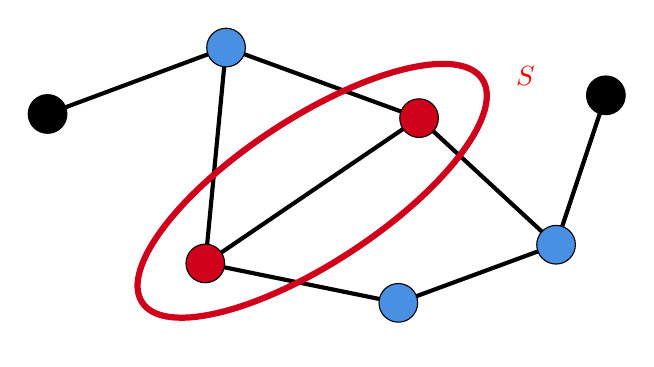
\begin{tikzpicture}[x=0.75pt,y=0.75pt,yscale=-1,xscale=1]
%uncomment if require: \path (0,300); %set diagram left start at 0, and has height of 300

%Shape: Circle [id:dp36255822406593574] 
\draw  [fill={rgb, 255:red, 0; green, 0; blue, 0 }  ,fill opacity=1 ] (98.21,120.31) .. controls (98.21,115.17) and (102.38,111) .. (107.52,111) .. controls (112.66,111) and (116.83,115.17) .. (116.83,120.31) .. controls (116.83,125.46) and (112.66,129.62) .. (107.52,129.62) .. controls (102.38,129.62) and (98.21,125.46) .. (98.21,120.31) -- cycle ;
%Straight Lines [id:da6762243021815164] 
\draw [line width=1.5]    (193.52,88.31) -- (107.52,120.31) ;
%Straight Lines [id:da5943065246596186] 
\draw [line width=1.5]    (193.52,88.31) -- (183.52,192.31) ;
%Straight Lines [id:da5922541880633836] 
\draw [line width=1.5]    (286.52,122.31) -- (193.52,88.31) ;
%Straight Lines [id:da5429713502318034] 
\draw [line width=1.5]    (286.52,122.31) -- (183.52,192.31) ;
%Straight Lines [id:da08272941688144808] 
\draw [line width=1.5]    (276.52,211.31) -- (183.52,192.31) ;
%Straight Lines [id:da7508692114128916] 
\draw [line width=1.5]    (352.52,183.31) -- (276.52,211.31) ;
%Straight Lines [id:da583686318615475] 
\draw [line width=1.5]    (286.52,122.31) -- (352.52,183.31) ;
%Shape: Ellipse [id:dp6095919685494009] 
\draw  [color={rgb, 255:red, 208; green, 2; blue, 27 }  ,draw opacity=1 ][line width=2.25]  (153.09,211.09) .. controls (142.55,195.02) and (170.68,157.93) .. (215.93,128.23) .. controls (261.18,98.53) and (306.41,87.47) .. (316.95,103.54) .. controls (327.49,119.6) and (299.36,156.7) .. (254.11,186.4) .. controls (208.86,216.1) and (163.64,227.15) .. (153.09,211.09) -- cycle ;
%Shape: Circle [id:dp6185527262442363] 
\draw  [fill={rgb, 255:red, 0; green, 0; blue, 0 }  ,fill opacity=1 ] (367.21,111.31) .. controls (367.21,106.17) and (371.38,102) .. (376.52,102) .. controls (381.66,102) and (385.83,106.17) .. (385.83,111.31) .. controls (385.83,116.46) and (381.66,120.62) .. (376.52,120.62) .. controls (371.38,120.62) and (367.21,116.46) .. (367.21,111.31) -- cycle ;
%Straight Lines [id:da2733414566463044] 
\draw [line width=1.5]    (352.52,183.31) -- (376.52,111.31) ;
%Shape: Circle [id:dp8390082539090082] 
\draw  [fill={rgb, 255:red, 208; green, 2; blue, 27 }  ,fill opacity=1 ] (174.21,192.31) .. controls (174.21,187.17) and (178.38,183) .. (183.52,183) .. controls (188.66,183) and (192.83,187.17) .. (192.83,192.31) .. controls (192.83,197.46) and (188.66,201.62) .. (183.52,201.62) .. controls (178.38,201.62) and (174.21,197.46) .. (174.21,192.31) -- cycle ;
%Shape: Circle [id:dp6411364120529555] 
\draw  [fill={rgb, 255:red, 208; green, 2; blue, 27 }  ,fill opacity=1 ] (277.21,122.31) .. controls (277.21,117.17) and (281.38,113) .. (286.52,113) .. controls (291.66,113) and (295.83,117.17) .. (295.83,122.31) .. controls (295.83,127.46) and (291.66,131.62) .. (286.52,131.62) .. controls (281.38,131.62) and (277.21,127.46) .. (277.21,122.31) -- cycle ;
%Shape: Circle [id:dp7676086263076403] 
\draw  [fill={rgb, 255:red, 74; green, 144; blue, 226 }  ,fill opacity=1 ] (184.21,88.31) .. controls (184.21,83.17) and (188.38,79) .. (193.52,79) .. controls (198.66,79) and (202.83,83.17) .. (202.83,88.31) .. controls (202.83,93.46) and (198.66,97.62) .. (193.52,97.62) .. controls (188.38,97.62) and (184.21,93.46) .. (184.21,88.31) -- cycle ;
%Shape: Circle [id:dp08773901760859015] 
\draw  [fill={rgb, 255:red, 74; green, 144; blue, 226 }  ,fill opacity=1 ] (267.21,211.31) .. controls (267.21,206.17) and (271.38,202) .. (276.52,202) .. controls (281.66,202) and (285.83,206.17) .. (285.83,211.31) .. controls (285.83,216.46) and (281.66,220.62) .. (276.52,220.62) .. controls (271.38,220.62) and (267.21,216.46) .. (267.21,211.31) -- cycle ;
%Shape: Circle [id:dp10937116699267224] 
\draw  [fill={rgb, 255:red, 74; green, 144; blue, 226 }  ,fill opacity=1 ] (343.21,183.31) .. controls (343.21,178.17) and (347.38,174) .. (352.52,174) .. controls (357.66,174) and (361.83,178.17) .. (361.83,183.31) .. controls (361.83,188.46) and (357.66,192.62) .. (352.52,192.62) .. controls (347.38,192.62) and (343.21,188.46) .. (343.21,183.31) -- cycle ;

% Text Node
\draw (332,96.4) node [anchor=north west][inner sep=0.75pt]    {$\textcolor{red}{S}$};
\end{tikzpicture}
\caption{An example of such function evaluation $f(\textcolor{red}{S}) = \textcolor{red}{2} + \textcolor{blue}{3} = 5$}
\label{fig:max-cover}
\end{figure}

As stated, this definition of the Max Cover problem tries to find at most $k$ nodes in a graph for which the corresponding set of nodes has the largest submodular value (the output of the submodular function). And the submodular value in the context of the max cover problem can intuitively be seen as a measure of coverage.
 
% \begin{itemize}
%     \item Erd˝os R´enyi. We generate $G(n, p)$ graphs with a $p = 0.01$ probability of each edge. Since many nodes have similar degree in this model and each node’s edges are spread randomly across the graph, a random set of nodes often achieves good coverage.
%     \item Stochastic block model. We generate SBM graphs with a $p = 0.1$ probability of an edge between each pair of nodes in the same cluster. Here, we expect that a good solution will cover nodes in all clusters.
%     \item Watts-Strogatz. We generate WS graphs initialized as ring lattices with 2 edges per node and a $p = 0.1$ probability of rewiring edges. In these ‘small-world’ graphs, many nodes have identical degree, so good solutions contain nodes chosen to minimize coverage overlaps.
%     \item Barb´asi-Albert. We generate BA graphs with $m = 1$ edges added per iteration. BA graphs exhibit scale-free structure and tend to have a small set of high-degree nodes. Therefore, it is often possible to obtain high coverage in these graphs by choosing the highest degree nodes.
% \end{itemize}

    % Max cover on synthetic graphs generated via four different well-studied graph models: Stochastic Block Model (SBM); Erd˝os R´enyi (ER); Watts-Strogatz (WS); and Barb´asi-Albert (BA)

\section{Algorithm 1: Fast Adaptive Sequencing Technique (\textsc{FAST})}
The first of the two algorithms we plan to consider for the Max Cover problem is a randomized parallel algorithm called FAST, which stands for Fast Adaptive Sequencing Technique~\cite{breuer2019fast}. The key idea behind this algorithm is the application of Adaptive Sequencing, which, as the name suggests, finds a solution by considering sequences of elements (or nodes in the case of the graph Max Cover problem). The technique works by randomly generating sequences of elements, after which it considers a prefix of the sequence that yields the highest submodular value. This process is iteratively applied wherein each iteration, the elements in the prefix yielding the highest marginal contributions are removed form the considered set. Additionally, elements with low marginal contributions are also removed in each iteration of the technique.    

FAST integrates Adaptive Sequencing with the binary search algorithm. Instead of checking every prefix, it only considers geometrically increasing prefixes of the considered set of elements. It then performs a left binary search to find the optimal prefix.

This modified adaptive sequencing technique is applied at two different levels of the FAST algorithm, which consists of two parts - a sequential outer search that spins off a number of parallel queries, and an inner search corresponding to each of these parallel queries. The outer search, referred to as the \textsc{FAST-FULL} algorithm (Algorithm~\ref{alg:fast-full}) initiates guesses of the optimal set to use as a metric for thresholding good marginal contributions in the corresponding query search. These guesses $v \in V$ of $\OPT$, the candidate optimal solution, are geometrically increasing over the modular contributions of the elements for sets of different sizes-ranging from $\max_{a \in N} f(a)$ to $\max_{|S| \leq k} \sum_{a \in S} f(a)$ by a $(1 - \varepsilon)^{-1}$ geometric factor. For this reason, $V$ will contain a value that is a $1- \varepsilon$ approximation to $\OPT$. Furthermore, this means that the overall search guarantees a solution $S$ that is a $1-1/e$ approximation to $v$.

In practice, however, a single iteration of this binary search is shown to be sufficient to achieve the approximation guarantee.

% We describe the \textsc{FAST-FULL} algorithm (Algorithm~\ref{alg:full}). The main part of the algorithm is the \textsc{FAST} subroutine (Algorithm~\ref{alg:main}), which is instantiated with different guesses of $\OPT$, which is the value of optimal solution. 
 
\begin{algorithm}[H]
\caption{\textsc{Fast-Full}: the full algorithm}
\begin{algorithmic}
    	\STATE \textbf{input} function $f$, cardinality constraint $k$, parameter $\varepsilon$
    	\STATE $V \leftarrow$ \textsc{Geometric}$(\max_{a \in N} f(a), \max_{|S| \leq k} \sum_{a \in S} f(a), 1 - \varepsilon)$
    	\STATE $v^{\star} \leftarrow$ \textsc{Binary-Search}$(V, \max\{v \in V: f(S_v) \geq (1 - 1/e)v\})$
    	\STATE \ \ \ \ \ where $S_v \leftarrow$ \textsc{FAST}$(v)$
    	\STATE \textbf{return} $S_{v^{\star}}$ 
  \end{algorithmic}
  \label{alg:fast-full}
\end{algorithm}

The inner search, referred to as the \textsc{FAST} subroutine (Algorithm~\ref{alg:main}), makes a few different considerations in the search for the optimal solution. While the constraints have not been met (namely, the constraint of at most $k$ elements and an upper bound on the number of iterations derived from the approximation guarantees, $\varepsilon^{-1}$), the subroutine computes the threshold $t$ from the given candidate optimal solution, OPT, and will use this threshold to determine what constitutes as a high marginal contribution when performing submodular optimization.

The subroutine then iteratively adds to the solution using both Vanilla Adaptive Sequencing, which process a randomly generated sequence $a_1, \ldots, a_{|X|}$ from the set $X$ and the modified Adaptive Sequencing technique that continues to process a sample of the remaining elements in $X$. The Vanilla Adaptive Sequencing is considered as the preprocesing step to help add to the solution elements guaranteed to have a high marginal contribution while aiding in removing elements with low marginal contributions from being considered any further.

The modified Adaptive Sequencing step will then perform a binary search over geometrically increasing prefix indices $i$ to identify a position $i^{\star}$ in this sequence corresponding to the prefix $A_{i^{\star} - 1}$. Position $i^{\star}$ is defined by~\cite{breuer2019fast} as the largest position such that there is a large fraction of elements in $X$ with high contribution to $S \cup A_{i^{\star} - 1}$ where $S$ is the current solution. This prefix, $A_{i^{\star}}$ is then added to the current solution $S$.

% \textsc{FAST} algorithm generates at every iteration a  uniformly random sequence $a_1, \ldots, a_{|X|}$ of the elements $X$ not yet discarded. After the preprocessing step which adds to $S$ elements guaranteed to have high contribution,the  algorithm  identifies a position $i^{\star}$ in this sequence which determines the prefix $A_{i^{\star} - 1}$ that is added to the current solution $S$. Position $i^{\star}$ is defined as the largest position such that there is a large fraction of elements in $X$ with high contribution to $S \cup A_{i^{\star} - 1}$. To find $i^{\star}$, we binary search over geometrically increasing positions $i \in I \subseteq [k]$. At each position $i$, we only evaluate the contributions of elements $a \in R$ , where $R$ is a uniformly random subset of $X$ of size $m$, instead of all elements $X$.  

\begin{algorithm}[H]
\caption{\algoptimized: the Fast Adaptive Sequencing Technique algorithm}
\begin{algorithmic}
    \STATE \textbf{input}  function $f$, cardinality constraint $k$, guess $v$ for $\OPT$, parameter $\varepsilon$
    \STATE 	 $S \leftarrow \emptyset $
    \STATE  \textbf{while} $|S| < k$ and number of  iterations  $< \varepsilon^{-1}$ \textbf{do}
    \STATE   \ \  $X \leftarrow N,  t \leftarrow (1-\varepsilon) (v - f(S))/k$
	\STATE   \ \ \textbf{while} $X \neq \emptyset$ and $|S| < k$  \textbf{do}
	\STATE  \ \ \ \   $a_1, \ldots, a_{|X|} \leftarrow \textsc{Sequence}(X, |X|), A_i \leftarrow a_1, \ldots, a_i$
	\STATE \ \ \ \   $S \leftarrow S \cup \{a_i : f_{S \cup A_{i-1}}(a_i) \geq t \}$
	\STATE \ \ \ \ $X_0 \leftarrow \{a \in X : f_{S}(a) \geq t\}$
	\STATE \ \ \ \   \textbf{if} $|X_0| \leq (1 - \varepsilon) |X|$ \textbf{then} $X \leftarrow X_0$ and continue to  next iteration
	\STATE \ \ \ \  $R \leftarrow \textsc{Sample}(X, m)$, $I \leftarrow \textsc{Geometric}(1, k - |S|, 1 - \varepsilon)$
    \STATE \ \ \ \  $i^{\star} \leftarrow$ \textsc{Binary-Search}$(I,  \max \{i  \in I : |\left\{a \in R : f_{S \cup A_{i-1}}(a) \geq   t \right\}| \geq (1 - 2 \varepsilon) |R|\})$ 
	\STATE \ \ \ \  $S \leftarrow S \cup A_{i^{\star} }$
    	\STATE \textbf{return} $S$
  \end{algorithmic}
  \label{alg:main}
\end{algorithm}
\section{Algorithm 2: Randomized Parallel Greedy}

We outline basic properties of a continuous extension of submodular functions to the fractional values in $[0,1]^{N}$ called the multilinear extension.

Denote a finite set $N$, and $f$ will be a set function defined over the power set of $N$.

\begin{equation}
    f: 2^{N} \rightarrow \mathbb{R}
\end{equation}
\begin{definition}[Multilinear extension]
The multilinear extension of $f$ is the function $F:[0,1]^{n} \rightarrow \mathbb{R}$ defined by:
\begin{equation}
    F(x)=\sum_{S \subseteq N} f(S) \prod_{i \in S} x_{i} \prod_{i \in N \backslash S}\left(1-x_{i}\right)
\end{equation}
\end{definition}
Let $x \vee y$ be the coordinatewise maximum of $x$ and $y$. We also write $F_y(x) = F (x \vee y) - F (y)$ which generalizes the definition of marginal values to the continuous setting.

There is a probabilistic interpretation of the multilinear extension. Given $x \in[0,1]^{n}$ we can define $X$ to be the random subset of $N$ in which each element $i \in N $ is included independently with probability $x_i$ and not included with probability $1 - x_i$. We write $X\sim x$ to say that $X$ is the random subset sampled according to $x$. Then the multilinear extension $F$ is simply:
\begin{equation}
    F(x)=\underset{X \sim x}{\mathbb{E}}[f(X)]
\end{equation}
For this reason, using the multilinear extension is often called relaxing through expectation.

Parallel Greedy is a straightforward parallelization of the original continuous-greedy algorithm due to Călinescu et al.~\cite{CGC11}, specialized to the cardinality polytope. Continuous-greedy is an iterative and monotonic algorithm that, in each iteration, computes the gradient $\nabla F(x)$ and finds the point $v$ in the constraint polytope that maximizes
$\left<\nabla F(x), v\right>$. 

Since we consider a model where we only have oracle access to the set function $f$, we use the alternative algorithm randomized-parallel-greedy, which is guided by the previous parallel-greedy algorithm, but maintains a discrete set $Q \subset N$ rather than a fractional solution $x$. The primary difference is in steps, where rather than add the fractional solution $\delta S$ to the solution, we first sample a set $R\sim\delta S$ (where each element in $S$ is drawn independently with probability $\delta$), and then we add $R$ to the running solution~\cite{chekuri2018submodular}.

The variable $t$ is used to track the expected cardinality of $|Q|$. One can simplify the algorithm by replacing the variable $t$ with $|Q|$ wherever it appears, and the analysis would generally still hold. The inclusion of $t$ makes the analysis more straightforward, as we can use $t$ to track progress throughout the algorithm.


Estimating OPT: The algorithm requires a value $\lambda$ that is an upper bound on OPT. Preprocessing allows us to choose $\lambda=\sum_{j} f(j)$ and we have $OPT \leq \lambda \leq n\cdot OPT$. It is also useful to have an estimate that is within a constant factor. This can be done by running the algorithm in parallel with $O(\log n)$ geometrically increasing values of $\lambda$ and picking the best solution from the parallel runs.

Let us describe the algorithm in more detail. At first, we initialize the variables and estimate the OPT (the search for the estimate is part of the preprocessing). Then we construct a set of candidates satisfying the condition (we want to select the elements so that their marginal values were greater than the average value for the optimum).

After that, we choose the largest $\delta$ that satisfies the condition that the expectation of the marginal value is large enough and that the cardinality constraint holds. Then we sample the subset and add to the solution, update the variables, and then continue the loop. When we exit the inner loop, we decrease the estimate of the optimal value and build a new set of candidates.

\begin{algorithm}[H]
\caption{Randomized Parallel Greedy}
\begin{algorithmic}
    	\STATE \textbf{input} function $f$, cardinality constraint $k$, parameter $\varepsilon$
\STATE$1 . Q \leftarrow \emptyset, t \leftarrow 0, \lambda \leftarrow \mathrm{OPT} / /$ or any $\lambda \geq \mathrm{OPT}$
\STATE 2. while $t \leq(1-2 \varepsilon) k$ and $\lambda \geq e^{-1}$ OPT
\STATE \quad A. let $S=\left\{j \in N: f_{Q}(j) \geq \frac{(1-\varepsilon) \lambda}{k}\right\}$
\STATE \quad B. while $S$ is not empty and $t \leq(1-2 \varepsilon) k$
\STATE \quad \quad i. chose $\delta$ maximal s.t.
\STATE \quad \quad \quad a. $F_{Q}(Q+\delta S) \geq(1-\varepsilon)^{2} \lambda \frac{\delta|S|}{k}$
\STATE \quad \quad \quad b. $t+\delta|S| \leq(1-2 \varepsilon) k$
\STATE \quad \quad ii. sample $R \sim \delta S$
\STATE \quad \quad iii. $Q \leftarrow Q \cup R, t \leftarrow t+\delta|S|$
\STATE \quad \quad iv. update $S$
\STATE \quad C. $\quad \lambda \leftarrow(1-\varepsilon) \lambda$
\STATE 3. return $Q$
  \end{algorithmic}
  \label{alg:full}
\end{algorithm}

\section{Theoretical guarantees}
% \textsc{FAST} obtains a $1-1/e-\epsilon$ approximation w.p. $1- \delta$ and that it has $\tilde{O}(\varepsilon^{-2} \log n)$  adaptive complexity and $\tilde{O}(\varepsilon^{-2} n +\varepsilon^{-4} \log(n)  \log(\delta^{-1}))$ query complexity.
\begin{theorem}[\textsc{FAST}~\cite{breuer2019fast}]
\label{thm:main_FAST} 
Assume $k \geq \frac{2 \log(2\delta^{-1} \ell)}{\varepsilon^2 (1 - 5\varepsilon)}$ and $\varepsilon \in (0, 0.1)$, where  $\ell = \log(\frac{\log k}{\varepsilon})$. Then, \textsc{FAST} with $m = \frac{2 + \varepsilon}{\varepsilon^2(1 -  3\varepsilon)} \log(\frac{4\ell\log n}{\delta \varepsilon^2})$ has at most $\varepsilon^{-2} \log(n)  \ell^2$  adaptive rounds,   
$2\varepsilon^{-2}  \ell n +  \varepsilon^{-2} \log(n) \ell^2 m$ queries, and achieves a $1 - \frac{1}{e} - 4 \varepsilon$ approximation 
w.p. $1 - \delta$.
\end{theorem} 

\begin{theorem}[\textsc{Randomized-Parallel-Greedy}~\cite{chekuri2018submodular}]
Let $\varepsilon>0$ be given, let $f: 2^{\mathcal{N}} \rightarrow \mathbb{R}_{\geq 0}$ be a normalized, monotone submodular function in the oracle model, and let $k \in \mathbb{N}$. Then with high probability, randomized-parallel-greedy computes a $(1-\varepsilon)\left(1-e^{-1}\right)$ multiplicative approximation to the maximum value set of cardinality $k$ with $O\left(\frac{\log n}{\epsilon^{2}}\right)$ expected adaptivity and $\tilde{O}\left(\frac{n}{\varepsilon^{4}}\right)$ expected oracle calls to $f$.
\end{theorem}

\begin{table}[h]
\begin{center}
\begin{tabular}{cll}\vspace{0.2cm}
        & \emph{Query complexity} & \emph{Adaptivity} &   \\\ \vspace{0.3cm}
        % \hline
%  Randomized-Parallel-Greedy
 \textsc{Randomized-Parallel-Greedy}~\cite{chekuri2018submodular}& $\mathcal{O}\left(  \frac{n}{\varepsilon^4}  \log\left(\frac{n}{\delta}\right) \log^2 n\right)  $ & $ \mathcal{O}\left(\frac{\log n}{\varepsilon^2}  \right)$ & \\\ \vspace{0.3cm}
  \textsc{FAST}~\cite{breuer2019fast} &     $\mathcal{O}\left(\frac{  n \ell}{\varepsilon^2} +  \frac{ \ell^2 \log n}{\varepsilon^4}   \log(\frac{\ell\log n}{\delta \varepsilon^2})\right)$        &   $\mathcal{O}\left(\frac{ \ell^2 \log n}{\varepsilon^2}\right)$   & 
\end{tabular}
  \caption{Comparison on the query complexity and adaptivity achieved in order to obtain a $1-1/e-\varepsilon$ approximation with probability $1 - \delta$, where  $\ell = \log\left(\frac{\log k}{\varepsilon}\right)$.  }
  \label{tab:queries}
\end{center}
\end{table}


\section{Experiments}

Since the objective of the Max Cover takes into account the connectivity of the nodes, we plan to test the considered algorithms on graphs which characteristically exhibit very different topologies. The types of synthetically generated graphs we plan on experimenting with are:
\begin{itemize}
    \item \emph{Stochastic Block Model} (SBM)
    \item \emph{Erd\H{o}s R\'{e}nyi} (ER)
    \item \emph{Watts-Strogatz} (WS)
    \item \emph{Barb\'{a}si-Albert} (BA)
\end{itemize}

\paragraph{Stochastic block model}
The stochastic block model takes the following parameters:
\begin{itemize}
    \item The number $n$ of vertices;
    \item a partition of the vertex set $\{1,\ldots,n\}$ into disjoint subsets $C_1,\ldots,C_r$, called 'communities';
    \item a symmetric $r \times r$ matrix $P$ of edge probabilities.
\end{itemize} 
The edge set is then sampled at random as follows: any two vertices $u \in C_i$ and $v \in C_j$ are connected by an edge with probability $P_{ij}$. An example problem is: given a graph with $n$ vertices, where the edges are sampled as described, recover the groups $C_1,\ldots,C_r$.

\paragraph{Erd\H{o}s R\'{e}nyi}
There are two closely related variants of the Erd\H{o}s R\'{e}nyi random graph model. In the $G(n,M)$ model, a graph is chosen uniformly at random from the collection of all graphs which have $n$ nodes and $M$ edges.  For example, in the $G(3,2)$ model, each of the three possible graphs on three vertices and two edges are included with probability $\frac{1}{3}$. 

In the $G(n,p)$ model, a graph is constructed by connecting nodes randomly. Each edge is included in the graph with probability $p$ independent from every other edge. Equivalently, all graphs with $n$ nodes and $M$ edges have equal probability of $p^M (1-p)^{{n \choose 2}-M}$.
The parameter $p$ in this model can be thought of as a weighting function; as $p$ increases from $0$ to $1$, the model becomes more and more likely to include graphs with more edges and less and less likely to include graphs with fewer edges. In particular, the case $p = 0.5$ corresponds to the case where all $2^\binom{n}{2}$ graphs on $n$ vertices are chosen with equal probability.

\paragraph{Watts-Strogatz}\\
Given the desired number of nodes $N$, the mean $K$ (assumed to be an even integer), and a special parameter $\beta$, satisfying $0 \leq \beta \leq 1$ and $N\gg K \gg \ln N \gg 1$, the model constructs an undirected graph with $N$ nodes and $\frac{NK}{2}$ edges in the following way:
\begin{itemize}
    \item Construct a regular ring lattice, a graph with $N$ nodes each connected to $K$ neighbors, $K/2$ on each side. That is, if the nodes are labeled  $0 \ldots {N-1}$, there is an edge $(i, j)$ if and only if $0 < |i - j|\ \mathrm{mod}\ \left( N-1-\frac K 2 \right) \leq \frac K 2.$
    \item For every node $i=0,\dots, {N-1}$ take every edge connecting $i$ to its $K/2$ rightmost neighbors, that is every edge $(i, j\ \mathrm{mod}\ N)$ with $i < j \leq i + K/2$, and rewire it with probability $\beta$. Rewiring is done by replacing $(i, j\ \mathrm{mod}\ N)$ with $(i, k)$ where $k$ is chosen uniformly at random from all possible nodes while avoiding self-loops ($k \ne i$) and link duplication (there is no edge $(i, {k'})$ with $k' = k$ at this point in the algorithm).
\end{itemize}

\paragraph{Barb\'{a}si-Albert}
The steps of the growth of the network according to the Barabasi–Albert model  ($m_0=m=2$).
The network begins with an initial connected network of $m_0$ nodes.

New nodes are added to the network one at a time. Each new node is connected to $m \le m_0$ existing nodes with a probability that is proportional to the number of links that the existing nodes already have. Formally, the probability $p_i$ that the new node is connected to node $i$ is 
$$p_i = \frac{k_i}{\sum_j k_j},$$

where $k_i$ is the degree of node $i$ and the sum is made over all pre-existing nodes $j$ (i.e. the denominator results in twice the current number of edges in the network). Heavily linked nodes ("hubs") tend to quickly accumulate even more links, while nodes with only a few links are unlikely to be chosen as the destination for a new link. The new nodes have a "preference" to attach themselves to the already heavily linked nodes.
\\

To test how well the algorithms perform on these graphs, we additionally plan on running experiments for different sample sizes of the graphs - to the extent the Ibex CPU clusters provided by KAUST can tolerate. Presumably starting at 500 nodes and scaling to higher sizes depending on the computational load our parallel setup can support.

\section{Implementation Plans}

For implementation, we have divided up the work to consist of data generation, algorithms implementation in Python, and setting up the support for testing parallelization.
For setting up the parallelization, we plan on using the Message Passing Interface (MPI) library, which allows handling the parallel communication between processors. This setup will need to be done on Ibex, which gives access to multiple CPUs.

\begin{table}[H]
    \begin{center}
        \begin{tabular}{||c c||} 
         \hline
         Date & Tasks \\
         \hline\hline
         2-8 November & Implement Synthetic Graph Generation  \\ 
         \hline
         9-15 November & Implement Randomized-Parallel-Greedy \\
         \hline
         16-22 November & Implement FAST algorithm  \\
         \hline
         23-29 November & Setup Ibex environment and Debug  \\
         \hline
         1-7 December & Run experiments and obtain results  \\
         \hline
         8-13 December & Prepare for project report and presentation  \\
         \hline
        \end{tabular}
    \caption{Preliminary schedule to meet our implementation goals.}
    \label{tab:schedule}
    \end{center}
\end{table}
\clearpage
% \tiny % \small
\begin{thebibliography}{99}
    \bibitem[NW78]{nemhauser1978best} 
    George~L Nemhauser and Laurence~A Wolsey.
	\newblock Best Algorithms for Approximating the Maximum of a Submodular Set Function.
	\newblock {\em Mathematics of Operations Research, 3(3):177--188},1978.
	
	\bibitem[NWF78]{NWF78}
    George~L Nemhauser, Laurence~A Wolsey, and Marshall~L Fisher.
    \newblock An analysis of approximations for maximizing submodular set functions.
    \newblock {\em Mathematical Programming, 14(1):265--294}, 1978.

    \bibitem[CQ19]{chekuri2018submodular} Chandra Chekuri and Kent Quanrud.
	\newblock Submodular Function Maximization in Parallel via the Multilinear Relaxation.
	\newblock \emph{Proceedings of the 2019 Annual ACM-SIAM Symposium on Discrete Algorithms, pp 303--322, 2019}

    \bibitem[BBY20]{breuer2019fast} A. Breuer, E. Balkanski, and Y. Singer
	\newblock The FAST Algorithm for Submodular Maximization.
	\newblock \emph{Proceedings of the 37th International Conference on Machine Learning}, 2020.
	
	\bibitem[BRS19]{BRS19} Eric Balkanski, Aviad Rubinstein, and Yaron Singer.
	\newblock An optimal approximation for submodular maximization under a matroid constraint in the adaptive complexity model.
	\newblock {\em STOC, pp 66--77}, 2019.
	
	\bibitem[CGC11]{CGC11} Calinescu, Gruia and Chekuri, Chandra and Pál, Martin and Vondrák, Jan
	\newblock Maximizing a Monotone Submodular Function Subject to a Matroid Constraint
	\newblock {\em SIAM J. Comput.~40, No. 6, pp. 1740--176}, 2011.
	
% 	\bibitem[Liu et al, 2020]{liu_fedsel_2020} R. Liu, Y. Cao, M. Yoshikawa, and H. Chen.
% 	\newblock FedSel: Federated SGD under Local Differential Privacy with Top-k Dimension Selection.
% 	\newblock \emph{Foundations and Trends in Theoretical Computer Science, 9(3–4):211–407, 2014.}

\end{thebibliography}

\end{document}
